\section{The G-MFRM Framework}
\label{sec:method}

Section~\ref{sec:confounding} established that omitting contamination from the measurement model produces directional bias in ability estimates (Observation~\ref{obs:ovb}). We now introduce the Gated Many-Facet Rasch Model (G-MFRM), which jointly estimates ability, judge severity, and contamination susceptibility within a single measurement framework. The key design choices, staged estimation with externally fixed exposure and a hierarchical HalfNormal prior for the contamination term, are motivated by the identifiability analysis in \S\ref{sec:identifiability} and the error propagation bounds in \S\ref{sec:error_prop}.

\subsection{Model Specification}
\label{sec:model_spec}

G-MFRM extends the standard MFRM \citep{linacre1989mfrm, linacre1994mfrm} by adding a multiplicative contamination gating term to the linear predictor (Eq.~\ref{eq:mfrm}):
%
\begin{equation}
\label{eq:gmfrm}
\log \frac{P(Y_{nij} \geq k)}{P(Y_{nij} < k)} = \theta_n - b_i - d_j - \gamma_k + c_n \cdot e_i,
\end{equation}
%
where all terms carry the definitions from Section~\ref{sec:confounding}. The gating structure $c_n \cdot e_i$ separates model-specific contamination susceptibility ($c_n \geq 0$) from item-specific exposure ($e_i \in [0,1]$). When $c_n = 0$ or $e_i = 0$, the gating term vanishes and Eq.~\ref{eq:gmfrm} reduces to the standard MFRM.

We enforce non-negativity and sparsity through a hierarchical HalfNormal prior: $\sigma_c \sim \text{HalfNormal}(1.0)$, $c^{\mathrm{raw}}_n \sim \text{HalfNormal}(1.0)$, $c_n = c^{\mathrm{raw}}_n \cdot \sigma_c$. The hierarchical structure provides adaptive shrinkage: when data support low contamination, $\sigma_c$ contracts toward zero. The remaining priors are $\theta_n \sim \mathcal{N}(0, 1)$, $b_i \sim \mathcal{N}(0, 1)$, $d_j \sim \mathcal{N}(0, 0.5)$, and uniform on $\gamma_k$.

G-MFRM extends the Doubly-Gated IRT model of \citet{shu2013dgirt} from binary gating to continuous exposure and multi-rater designs, and contributes the first formal identifiability conditions for gated IRT parameters (Propositions~\ref{prop:no_new}--\ref{prop:exposure_variation}, Theorem~\ref{thm:sufficient}) and error propagation bounds for staged estimation (\S\ref{sec:error_prop}).

\subsection{Staged Estimation}
\label{sec:staged}

Joint estimation of all parameters in Eq.~\ref{eq:gmfrm}, including $e_i$, would require identifying the bilinear product $c_n \cdot e_i$ from response data alone. This creates a fundamental non-identifiability (Proposition~\ref{prop:exposure_variation}). We resolve this through a three-stage procedure that fixes exposure externally before estimating the contamination parameters.

\paragraph{Stage 1: Standard MFRM.} We fit the standard MFRM (Eq.~\ref{eq:mfrm}) via the No-U-Turn Sampler (NUTS; \citealp{betancourt2015}) to obtain initial estimates $(\hat{\theta}, \hat{b}, \hat{d})$. These serve as warm-start values for the sampler in Stage~3 and improve convergence.

\paragraph{Stage 2: Exposure estimation.} Per-item exposure $e_i$ is estimated from external evidence independent of the response data. The primary signal is \emph{reference model anchoring} (75\% weight): win-rate residuals against a fixed anchor (gpt-4-0314) flag items where target models outperform difficulty-adjusted expectations. The secondary signal is \emph{cross-model agreement} (25\%): uniformly high scores across diverse architectures suggest exposure rather than easiness. The composite is clipped to $[0, 1]$ and fixed in Stage~3. Estimation is non-circular: $e_i$ is item-level while $c_n$ is model-level, and ablation with 100\% anchoring yields $\rho = 0.998$ (Appendix~\ref{app:weight_robustness}).

\paragraph{Stage 3: Joint MCMC.} With $e_i$ fixed, we sample $(\theta_n, b_i, d_j, c_n)$ jointly via NUTS. The priors are as specified in \S\ref{sec:model_spec}. The hierarchical contamination prior decomposes as
%
\begin{align}
\label{eq:contam_prior}
\sigma_c &\sim \text{HalfNormal}(1.0), \quad c^{\mathrm{raw}}_n \sim \text{HalfNormal}(1.0), \nonumber \\
c_n &= c^{\mathrm{raw}}_n \cdot \sigma_c,
\end{align}
%
where $\sigma_c$ is a shared global scale that governs the overall contamination magnitude. This non-centered parameterization improves sampler geometry by decoupling the global scale from the per-model effects.

Convergence is assessed via rank-normalized split-$\hat{R}$ \citep{vehtari2021rhat} and bulk effective sample size (ESS), with thresholds $\hat{R} < 1.05$ and ESS$_{\mathrm{bulk}} > 100$ following standard practice \citep{gelman2013bda}.\footnote{Synthetic validation with $N = 50$, $I = 100$, $J = 8$ yields satisfactory convergence across all parameters. Full diagnostic tables are reported in Section~\ref{sec:experiments}.}


\begin{figure}[t]
\centering
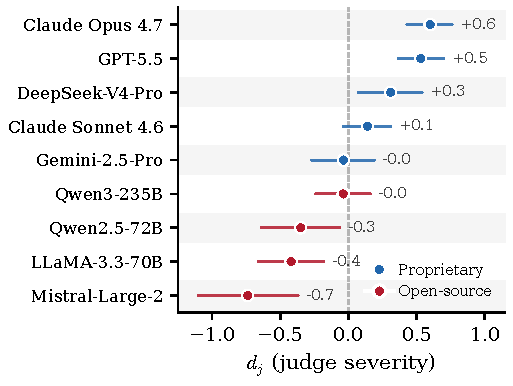
\includegraphics[width=\columnwidth]{forest_dj}
\caption{Judge severity estimates ($d_j$) with 95\% credible intervals for the full 9-judge panel ($N = 8$ analysis). Positive values indicate stricter scoring; the severity range spans 1.34 logits. The $N = 17$ analysis (\S\ref{sec:setup}) uses a 6-judge subset selected for item coverage.}
\label{fig:judge_severity}
\end{figure}

\subsection{Identifiability}
\label{sec:identifiability}

We establish that fixing $e_i$ externally is both necessary and sufficient for identifying the contamination parameters. All proofs assume $\sum_n \theta_n = 0$.

\begin{proposition}[No New Indeterminacy]
\label{prop:no_new}
When $e_i$ is fixed externally, $c_n \cdot e_i$ introduces no additional location or scale indeterminacy beyond the standard MFRM.
\end{proposition}

\begin{proposition}[Exposure Variation Necessary]
\label{prop:exposure_variation}
If $e_i = e$ for all $i$ (constant exposure), then $c_n$ and $\theta_n$ are not separately identifiable; hence $\mathrm{Var}(e_i) > 0$ is necessary.
\end{proposition}

Proofs are in Appendix~\ref{app:prop_proofs}.

\begin{theorem}[Sufficient Conditions for Local Identifiability]
\label{thm:sufficient}
G-MFRM is locally identifiable if: (i) a connected observation design, (ii) $J \geq 2$ judges, (iii) each model observes items with at least two distinct exposure values, and (iv) $\sum_n \theta_n = 0$.
\end{theorem}

The proof (Appendix~\ref{app:proof}) follows \citet{rothenberg1971} and establishes Fisher information non-singularity via the Cauchy--Schwarz inequality on the $(\theta_n, c_n)$ submatrix. Monte Carlo validation confirms successful $c_n$ recovery (Appendix~\ref{app:cn_recovery}).

\subsection{Error Propagation}
\label{sec:error_prop}

Treating Stage~2 estimates $\hat{e}_i$ as fixed creates a generated regressors problem \citep{pagan1984}. Let $\hat{e}_i = e_i + \epsilon_i$ with $\epsilon_i \sim \mathcal{N}(0, \sigma^2)$. The attenuation factor is $\lambda(\sigma) = \mathrm{Var}(e_i) / [\mathrm{Var}(e_i) + \sigma^2]$, reaching 50\% at $\sigma \approx 0.2$ in our setting ($\mathrm{Var}(e_i) \approx 0.04$). Empirically, $\theta$-RMSE increases by only 5.9\% and $c_n$-RMSE by 7.9\% below this threshold; beyond it ($\sigma = 0.5$), degradation becomes severe (Table~\ref{tab:error_prop}, Appendix~\ref{app:error_prop}). We apply the Murphy--Topel correction \citep{murphy1985} for honest credible intervals (Appendix~\ref{app:murphy_topel}).

\subsection{Fair Scores and Diagnostics}
\label{sec:fair_scores}

The Stage~3 posterior mean of $\theta_n$ provides a bias-and-contamination-corrected ``fair score'' for each model. The remaining parameters serve complementary diagnostic roles: per-model $c_n$ flags candidates for training data audit, per-judge $d_j$ informs judge calibration, and per-item $e_i$ identifies items for retirement or replacement.
